%-*- coding: UTF-8 -*-
% 论文总结.tex
% 2020年7月第二周
\documentclass[UTF8]{ctexart}
\usepackage{graphicx}
\usepackage{float}
\usepackage{amsmath}
\usepackage{geometry}
\geometry{a4paper,centering,scale=0.8}
\usepackage[format=hang,font=small,textfont=it]{caption}
\usepackage[nottoc]{tocbibind}
\usepackage{url}
\usepackage{listings}
\usepackage{booktabs}
\usepackage{xcolor}     %高亮使用的颜色
\definecolor{commentcolor}{RGB}{85,139,78}
\definecolor{stringcolor}{RGB}{206,145,108}
\definecolor{keywordcolor}{RGB}{34,34,250}
\definecolor{backcolor}{RGB}{220,220,220}

\lstset{
 columns=fixed,       
 numbers=left,                                        % 在左侧显示行号
 numberstyle=\tiny\color{gray},                       % 设定行号格式
 frame=none,                                          % 不显示背景边框
 backgroundcolor=\color[RGB]{245,245,244},            % 设定背景颜色
 keywordstyle=\color[RGB]{40,40,255},                 % 设定关键字颜色
 numberstyle=\footnotesize\color{darkgray},           
 commentstyle=\it\color[RGB]{0,96,96},                % 设置代码注释的格式
 stringstyle=\rmfamily\slshape\color[RGB]{128,0,0},   % 设置字符串格式
 showstringspaces=false,                              % 不显示字符串中的空格
 language=c++,                                        % 设置语言
}

\newenvironment{myquote}
{\begin{quote}\kaishu\zihao{-5}}
{\end{quote}}

\newcommand\degree{^\circ}

\title{\heiti Cognitive security for personal devices}
\author{\kaishu allen}
\date{\today}

\bibliographystyle{plain}

\newtheorem{thm}{定理}

\begin{document}
    
    \maketitle

    \clearpage
    \section{摘要}\label{sec:diyijie}
  	本文从三个研究角度在个人设备上创建认知性安全( cognitive security)。
    \begin{itemize}
    \item[*] 印记 和 连续部署的多模态生物识别技术 (imprinting and continuously deployed multimodal biometrics )
    \item[*] 通过虚拟化和可信计算实现的自我保护(self-protection through virtualization and trusted computing)
    \item[*] 可调节的自治安全 (adjustably autonomous security)
    \end{itemize}
	\clearpage
    \section{区分用户}\label{sec:dierjie}
    如何区分所有者和其他用户。第一,设备应当通过不断测量生物特征来识别用户。第二,没有用户可以设定所有者身份。设备应当给第一个用户留下足够丰富的印象。如同动物的印随现象。
    \subsection{识别所有者}
    传统的设备识别所有者主要是依靠挑战/应答的模式。设备发起挑战,所有者进行应答。例如:密码、生物特征以及硬件密钥。而人类,通常使用一些非隐私性、非机密性的特征来识别他人。例如:面部表情、面部结构、声音和步态。 
    \subsubsection{持续部署的生物识别技术( Continuously Deployed Biometrics)}
    在设备与所有者之间,我们可以根据持续的识别技术, 使设备保持对所有者的正面认证。攻击者必须要模仿所有者所有的认证因素才有可能模仿成功。我们验证的很多,例如:
    \begin{itemize}
    \item[*] 摄像头:面部,身高,姿势,身体形状,头发,肤色,眼睛颜色,运动模式
    \item[*] 麦克风:语音,音调,说话的模式
    \item[*] 键盘:输入的速度和暂停的模式
    \item[*] 定位设备:移动速度,点击的速度和频率
    \item[*] 计步器:步行速度,姿势变化
    \item[*] 使用模式:音乐选择,常用网站,常用的单词短语,每天的上网时间
    \item[*] 其他传感器:心率,体温,电导率。
    \end{itemize}
    上述特征并不能达到密码的强一致性,但是总体上讲,他可以提供足够的信息去验证用户。机器学习领域出现了很多弱分类器构建强分类器的问题。( Yoav Freund and Robert E. Schapire. A decisiontheoretic generalization of on-line learning and an application to boosting)攻击者需要投入大量成本去研究所有者所有的特征才能有一定机会攻击成功。因此攻击者可能会采取其他的攻击方式。
    \subsubsection{可用性}
    这种技术在设备与所有者之间交互较为频繁的时候可用,如果交互较少,建议使用密码或者挑战相应的机制。
    \subsection{在设备中印刻用户( Imprinting)}
    在设备与用户第一次接触的过程中,应当使用尽可能多的不同方式识别用户,并将其结果保存在受保护的存储环境中,即使是用户本人也无法对其进行修改。在一工作之后,用户应当相信攻击者无法损害这种认证关系。
    \subsubsection{可用性}
    设备需要实现一个细粒度的访问控制,用以不同角色用户的权限管理。

    当设备需要转换所有者时,设备需要重新初始化自己重新印刻。这一种改变的难度取决于设备的类型。
	\clearpage
	\section{架构}\label{sec:disanjie}
    对于人类而言,安全可以分为三个层次。头、心脑血管以及输入输出类型的身体安全,人体思想的安全和认知私密性和其他人际关系的保护。对于计算机而言,设备既需要保护自身的安全,同时要满足拥有者的意愿。故此,我们需要构建一种可信环境来运行可能存在危害的程序。

    如图1描述的安全可信架构所示,计算机的可信计算模块需要构建在一个可信平台模块(TPM, trusted platform module)之上,虚拟机需要建立在可信的虚拟机监控模块(VMM,virtual machine monitor)之上,安全管理模块中运行的虚拟机可以运行不受信任的代码,并用来检测这部分代码是否存在恶意行为。
    \begin{figure}[ht]
        \centering
        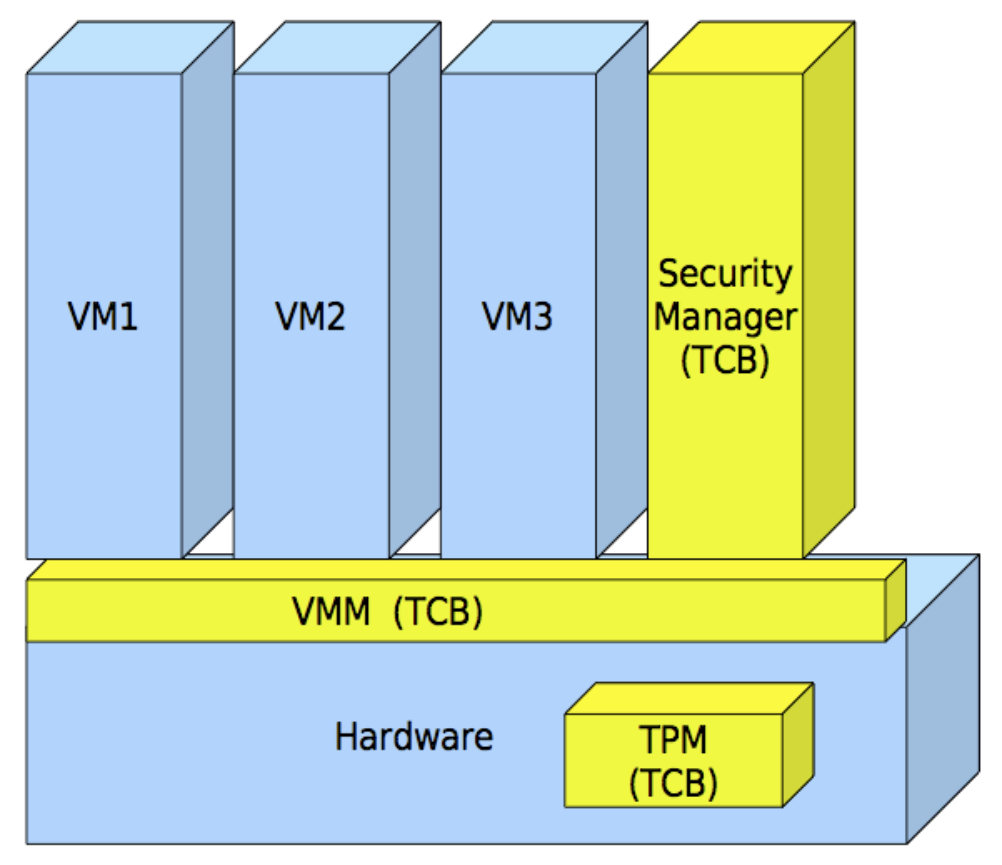
\includegraphics[scale=0.5]{picture/architecture.jpg}
        \caption{Figure 1: An illustration of the architecture for Abacus. }
        \label{fig:architecture}
    \end{figure}
    The trusted computing base (TPM, VMM, and security manager) is shown in yellow. The rest of the hardware is untrusted, as are the other virtual machines for running  applications.
    \subsection{可信计算}
    可信计算主要的优势在于提供攻击隔离。即使在软件受损的情况下也能够保证计算机中密钥的安全性。主要通过在计算机中建立信任链来完成。
    
    可信计算的由TCP(Trusted Computing Group,TCP)和微软的 Next Generation Secure Computing Base(NGSCB)推动并开发。
    
    可信计算通过测量机器上的每个层级结构(从BIOS和固件到操作系统和应用程序),将其结果的hash值存储在TPM中,从而实现安全启动。当控制权转移到下一个层级之前,会对这些度量进行检查,这些度量可用于保证安全关键代码不会被恶意更改。任何时候进行软件或者硬件的配置,必须重新建立信任链。
    
    虚拟化,提供了一种使用软件来增加额外灵活性和隔离的方法。
    \subsection{虚拟化}
虚拟化最极端的情况是仿真,所有的硬件都是抽象的。比较轻量级的情况是只有系统调用和驱动是抽象的。其安全收益主要是通过软件隔离实现的,软件可以在不同安全级别的环境下运行自己的虚拟机。假设管理虚拟机的VMM是安全的,那么各个虚拟机之间便是安全的。

    安全管理器,在整个架构的最顶层运行,以便保证VMM更加轻便不出错。安全管理器可以对其他虚拟机中应用程序的安全性和完整性的检测,并生成虚拟机。
    \begin{itemize} 
    \item[*] Stealthy malware detection through vmm-based ”out-of-the-box” semantic view reconstruction.  虚拟机状态检测
    \item[*] The ghost in the browser: Analysis of web-based malware 恶意代码检测
    \end{itemize}
    通过良好的虚拟化技术,可以保证拥有者在运行可以代码时,不需要接收安全提示,同时设备也不会受到安全威胁。
	\clearpage
	\section{可调控的自主安全性}\label{sec:disijie}
	设备需要明白拥有者的意图。比如说,钱很重要、不要发送垃圾邮件。但是设备并不知道拥有者是否故意发送垃圾邮件,以及是否确定要花钱。
    \begin{itemize} 
    \item[*] Principles of mixed-initiative user interfaces. 协作计划
    \item[*] Estimating information value in collaborative multi-agent planning systems. 可调自主
    \end{itemize}
    设备需要有一个内置知识库作为最基本的判断,然后再与拥有者进行交互的同时进行学习,建立新的模型,然后规定最终的安全行为。
    最后一步,设备需要考虑良好的界面。用户可能会因为不友好的安全提示而关闭安全性选项。
    \clearpage
	\section{结论}\label{sec:diwujie}
    \begin{itemize} 
    \item[*] 可信计算和虚拟化 :保护设备完整性
    \item[*] 持续部署的多模生物识别技术:所有者和设备之间的相互认证
    \item[*] 类似于人类的安全模型:负责任的进行安全决策
    \end{itemize}
    我们最终目的是在拥有者和设备之间建立更加良好的信任关系。
	\clearpage
	\bibliography{test}
\end{document}

